%*****************************************
\chapter{Design}
\label{ch:design}
%*****************************************

%\hint{This chapter should describe the design of the own approach on a conceptional level without %mentioning the implementation details. The section should have a length of about five pages.}
%The following section describes the process of this thesis from a high-level point of view. First, all %tasks performed before, during, or after the experiments are described. Afterward, these components are %used to describe the four experiments carried out for this thesis. For each experiment, a subsection %specifies its components and explains any choices made concerning hyperparameters.
The following section describes the process of this thesis from a high-level point of view. First, we define the components that describe an experiment. The subsequent sections specify these components for each experiment, respectively.


\section{Components}
With the following component structure, we intend to concisely communicate all parameters to understand and reproduce the presented experiments. For each experiment, we record the following components:
\begin{itemize}
	\item \textbf{Aim of the Experiment}\\
	The performed experiments pursued different goals. This component records the motivation of the given experiment and thus prepares the evaluation found in chapter \ref{ch:evaluation}.\\
	\item \textbf{Dataset and Preprocessing}\\
	We deployed three different datasets during this thesis. While chapter \ref{ch:datasets} provides a more detailed description, this component concisely specifies the type and shape of data points the experiment handles. Additionally, we note any preprocessing applied to the data before our experiment.\\
	\item \textbf{Task}\\
	A dataset embodies the experience of a given network, but the task researches expect their architecture to solve may still differ. A collection of text, for example, could either be classified by one network or translated by another. The task primarily formulates expectancies on the structure of a network's output, but it also has a significant influence on its architecture. Different tasks might also vary in difficulty.\\
	\item \textbf{Architecture}\\
	An accurate description of a network's architecture is vital to the reproducibility of any experiment. This component contains all parameters necessary to implement the network structure at hand in our framework and presents them in the shape of chapter \ref{background}. Any parameters that we inferred because we could not discern them from the referenced papers are mentioned here.
	J. Frankle and M. Carbin recorded the number of weights present in their architectures, which we utilized to check our implementation. In one case, where our number of weights partially disagree, we suggest possible explanations.\\
	\item \textbf{Training}\\  
	During training, a network repeatedly classifies small collections of data-points, called \textbf{batches}. After each batch, the framework calculates the momentary classification error and updates the weights, thus concluding a \textbf{training iteration}. This kind of training forms a numerical optimizations algorithm and, as such, might not converge after utilizing each data point just once. A training pass over all data points is called an \textbf{epoch}, and networks usually absolve it more than once. Our framework defines training in terms of epochs in contrast to J. Frankle and M. Carbin, who visualized their results in terms of iterations. For this reason, this component supplies the conversion rate between the two.\\
	\item \textbf{Pruning}\\  
	In their paper, J. Frankle and M. Carbin used different pruning percentages for different kinds of layers. Additionally, their results show that the quality of different architectures degrades at different speeds.\cite{LTH}
	For this reason, we employ different numbers of pruning iterations for the experiments and record them in this component alongside any remaining information on the training the architectures absolve.\\
\end{itemize}

\section{Reproduction: Dense Network | MNIST-Lenet-FCN}
\subsection*{Aim of the experiment}
The fully-connected Lenet network embodies the most basic architecture in the Lottery Ticket Hypothesis paper. Its reconstruction serves as a minimal working prototype for the codebase.
\subsection*{Dataset and Preprocessing}
For this experiment, we utilized the same data as J. Frankle and M. Carbin; the image set MNIST. It contains gray-scale images of hand-written digits with a size of 28x28 pixels.
We applied no preprocessing and utilized no data augmentation on the MNIST dataset.
\subsection*{Task and Architecture}
The task J. Frankle and M. Carbin. chose for their research is topic classification. The network is expected to return a ten-dimensional one-hot-encoding recording the digit displayed on the image in question.

\begin{tabularx}{\textwidth}[!h]{X X X}
	\multicolumn{3}{c}{\textbf{MNIST-Lenet-FCN Architecture}}
	\\
	\hline
	\endhead
	\textbf{Defaults} & Dense: activation & rectified linear unit\\
	\hline
	\textbf{Input} & output dimension & [28|28]\\
	[8pt]
	\textbf{Flatten} & output dimension & 784\\
	[8pt]
	\textbf{Dense} & output dimension & 300\\
	[8pt]
	\textbf{Dense} & output dimension & 100\\
	[8pt]
	\textbf{Dense} & output dimension & 10\\
	& activation & softmax\\
	\hline
\end{tabularx}

\subsection*{Training and Pruning}
\begin{tabularx}{\textwidth}[!h]{X X X}
	\multicolumn{3}{c}{\textbf{MNIST-Lenet-FCN Schedule}}
	\\
	\hline
	\endhead
	\textbf{Training} & epochs & 50\\
	& iterations per epoch & 1000\\
	& batch size & 60\\
	& loss & categorical crossentropy\\
	& optimizer & Adam\\
	& learning rate & $1.2 \cdot 10^{-4}$\\
	\hline
	\textbf{Pruning} & layers & Dense\\
	& amount & 20\%\\
	& iterations & 25\\
	& initial weights & 266.610\\
	& remaining weights & \textasciitilde1007\\
	\hline
\end{tabularx}

\section{Reproduction: Convolutional Network | CIFAR10-Conv6}
The Conv-6 architecture J. Frankle and M.Carbin developed for their paper, utilizes an additional popular kind of trainable layer, the convolutional layer, and has an order of magnitude more weights than the fully-connected Lenet architecture. Furthermore, it operates on an arguably more difficult dataset, CIFAR10. 

\subsection*{Aim of the Experiment}
The reproduction of the result they present for Conv-6 is a strong argument for the validity of our network concerning convolutional layers and more challenging datasets. 

\subsection*{Dataset and Preprocessing}
For this task, we utilized the image dataset CIFAR10, as did J. Frankle and M. Carbin. In contrast to MNIST, CIFAR10 contains colored images with a size of 32x32 pixels. Three gray-scale images encode an image's color's share of red, blue, and green, respectively. The result is the final size of 3x32x32 pixels.
The CIFAR10 dataset was neither preprocessed nor enhanced.

\subsection*{Task and Architecture}
As for the previous experiment, the task is image classification. While the number of classes remains the same as for MNIST, the complexity of possible objects increases, as they are composed of real-world objects, such as horses and cars.\\
\\
J. Frankle and M. Carbin developed Conv-6 based on the VGG architectures and only note the parameters necessary to infer the remaining parts of the infrastructure.\cite{LTH} We based our implementation on those parameters and the referenced paper of K. Simonyan and A. Zisserman.\cite{VGG}\\
After Inference, the number of weights in our dense part differs from the number reported by J.Frankle and M.Carbin. Because they do not supply an openly accessible implementation of their experiments, it was not possible to cross-validate the code.
As our framework employs the canonical way to prepare a multidimensional input for a dense layer, a flattening layer, we assume that J. Frankle and M. Carbin either reported the wrong layer parameters or the wrong number of weights in their description.
\newpage 
	%\begin{tabularx}{\textwidth}[!h]{!{\vrule width 2pt}X|X|X!{\vrule width 2pt}}
	\begin{tabularx}{\textwidth}[!h]{X X X}
		% \caption{MNIST-Lenet-FCN}
		\multicolumn{3}{c}{\textbf{CIFAR10-Conv6 Architecture}}
		\\
		\hline
		\endhead
		\textbf{Defaults} & \textbf{Dense}: activation & rectified linear unit\\
		& \textbf{2D Convolution}: activation & rectified linear unit\\
		& \textbf{2D Convolution}: kernel size & [3|3]\\
		& \textbf{2D Convolution}: edge padding & same\\
		& \textbf{2D Max Pooling}: pool size & [2|2]\\
		& \textbf{2D Max Pooling}: strides & [2|2]\\
		%\noalign{\hrule height 2pt}
		\hline
		\textbf{Input} & output dimension & [32|32|3]\\
		[8pt]
		\textbf{2D Convolution} & number of filters & 64\\
		& output dimension & [32|32|64]\\
		[8pt]
		\textbf{2D Convolution} & number of filters & 64\\
		& output dimension & [32|32|64]\\
		[8pt]
		\textbf{2D Max Pooling} & output dimension & [16|16|64]\\
		[8pt]
		\textbf{2D Convolution} & number of filters & 128\\
		& output dimension & [16|16|128]\\
		[8pt]
		\textbf{2D Convolution} & number of filters & 128\\
		& output dimension & [16|16|128]\\
		[8pt]
		\textbf{2D Max Pooling} & output dimension & [8|8|128]\\
		[8pt]
		\textbf{2D Convolution} & number of filters & 256\\
		& output dimension & [8|8|256]\\
		[8pt]
		\textbf{2D Convolution} & number of filters & 256\\
		& output dimension & [8|8|256]\\
		[8pt]
		\textbf{2D Max Pooling} & output dimension & [4|4|256]\\
		[8pt]
		\textbf{Flatten} & output dimension & 4096\\
		[8pt]
		\textbf{Dense} & output dimension & 256\\
		[8pt]
		\textbf{Dense} & output dimension & 256\\
		[8pt]
		\textbf{Dense} & output dimension & 10\\
		& activation & softmax\\
		\hline
	\end{tabularx}

\subsection*{Training and Pruning}
\begin{tabularx}{\textwidth}[!h]{X X X}
	% \caption{MNIST-Lenet-FCN}
	\multicolumn{3}{c}{\textbf{CIFAR10-Conv6  Schedule}}
	\\
	\hline
	\endhead
	%\noalign{\hrule height 2pt}
	%\noalign{\hrule height 2pt}
	\hline
	\textbf{Training} & epochs & 36\\
	& iterations per epoch & \textasciitilde833\\
	& batch size & 60\\
	& loss & categorical cross entropy\\
	& optimizer & Adam\\
	& learning rate & $3 \cdot 10^{-4}$\\
	\hline
	\textbf{Pruning} & layers & Dense\\
	& & 2D Convolution\\
	& iterations & 25\\
	& rate per iteration & 20 \%\\
	& & 15 \%\\
	& weighted rate & 17,46 \%\\
	& initial weights & 1.117.194\\
	& & 1.145.408\\
	& remaining weights & \textasciitilde4220\\
	& & \textasciitilde19698\\
	\hline
	%\noalign{\hrule height 2pt}
\end{tabularx}

%-----

\section{Transfer: Newsgroups-End2End}

\subsection*{Aim of the Experiment}
J. Frankle and M. Carbin report a desirable degree of pruning through the search for lottery tickets, but all their results pertain only to the field of image recognition. This experiment aspires to be a proof-of-concept for the search for lottery tickets in natural language applications. To this end, the code reproduces the network of an approach, of R. Pappagari et al.,  that achieved performance close to the state-of-the-art on a natural language processing task.\cite{End-to-End-CNN}\\
The architecture already performed quite well without the specific cost function they developed. To avoid problems with unique features and to increase the applicability of our findings, we omitted the special cost function. While the accuracy of our implementation dropped about ten percentage points, it still comes closer to the respective state-of-the-art than the Conv-6 architecture previously discussed.

\subsection*{Dataset and Preprocessing}
The natural language dataset used for this experiment is called "20 Newsgroup". It contains articles of varying lengths in plain text. As networks only handle numerical values, the documents had to be quantified. R. Pappagari et al. one-hot-encoded the documents on a word level, utilizing the vocabulary provided on the 20 newsgroup website.\footnote{
	The vocabulary length they documented does not agree with the length of the vocabulary provide at the website, which might be due to an update from the website's author. 
}\cite{End-to-End-CNN} 
Otherwise, they only mention that they used the canonical split of training and test data, which is not sufficient to accurately define the setup. First, the documents should be stripped of any metadata. Afterward, a tokenizer, of which many different ones exist, is necessary to split the articles into single words. The code provided along this thesis utilizes the word tokenizer supplied by the framework nltk. Furthermore, the provided vocabulary does not contain all tokens. For this experiment, we implicitly interpreted all tokens not referenced in the vocabulary as stopwords and omitted them.\\
Lastly, the input length of a network cannot be variable. While a few documents have an extreme length of over 3000, most of them do not. Simple zero-padding would overexert computer memory and overparametrize the architecture. Figures \ref{fig:Cut-Training} and \ref{fig:Cut-Training} show the document length histograms of test and training split for 20Newsgroups, respectively. Our computation devices were able to support a few hundred tokens per document, dependant on the number of pruning iterations. Ten pruning iterations are necessary to achieve a competitive pruning rate and left us with about 200 hundred tokens per document. The red line visualizes the cut-off. It leaves about 70 percent of the documents untruncated.

\begin{figure}
	\centering
	\begin{minipage}{0.45\textwidth}
		\centering
		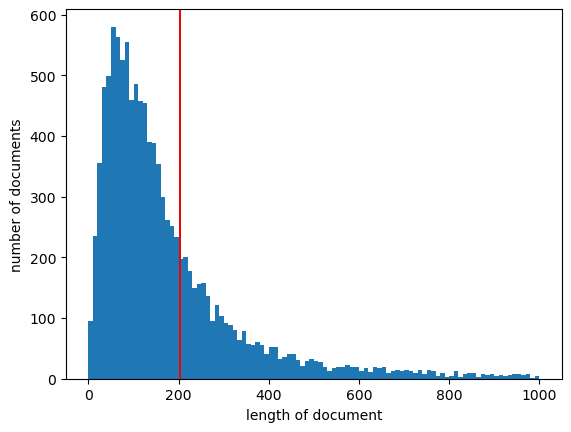
\includegraphics[height=180px]{gfx/4-Design/cut_training.png}
		\caption{Histogram of 20Newsgroups training data with cut-off}
		\label{fig:Cut-Training}
	\end{minipage}\hfill
	\begin{minipage}{0.45\textwidth}
		\centering
		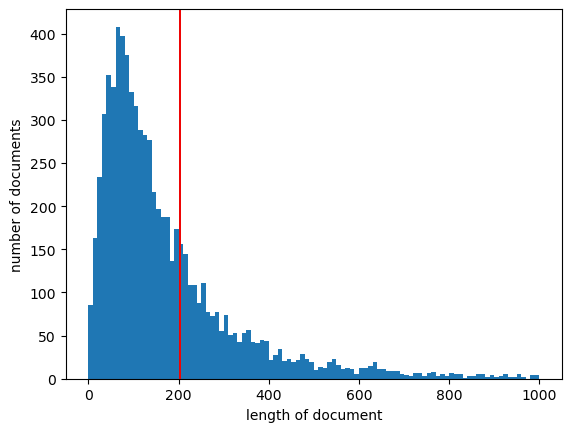
\includegraphics[height=180px]{gfx/4-Design/cut_test.png}
		\caption{Histogram of 20Newsgroups test data with cut-off}
		\label{fig:Cut-Test}
	\end{minipage}
	\vspace{7pt}
	\footnotesize{ 
		\\
		Source:\\
		These figure were produced by the author.
	}
\end{figure}


\subsection*{Task and Architecture}
Each document in the 20Newsgroups dataset was collected in a Usenet repository with an associated topic. For each document, the architecture returns its topic in a 20-dimensional one-hot-encoding.\\
\\
The Newsgroups-End2End ensemble combines 16 very similar embedding architectures. First, each network employs a trainable word-embedding layer to reduce the dimensionality of the one-hot-encoded word tokens. Subsequently, a convolutional layer and a few processing layers embed the whole document into a three-dimensional space. The overarching ensemble then collects the three remaining features of each architecture and classifies them with a dropout-regularized dense layer. Figure \ref{fig:Embedding-Network} and \ref{fig:Ensemble} display the single architectures and the ensemble, respectively.
\begin{figure}
	\centering
	\begin{minipage}{0.5\textwidth}
		\centering
		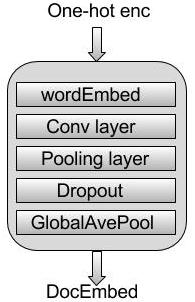
\includegraphics[height=180px]{gfx/4-Design/base_module.png}
		\caption{Layers of one embedding network}
		\label{fig:Embedding-Network}
	\end{minipage}\hfill
	\begin{minipage}{0.5\textwidth}
		\centering
		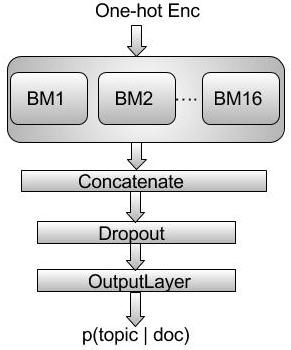
\includegraphics[height=180px]{gfx/4-Design/combined_model.png}
		\caption{Architecture of the whole network ensemble}
		\label{fig:Ensemble}
	\end{minipage}
	\vspace{7pt}
	\footnotesize{ 
		\\
		Source:\\
		"Joint Verification-Identification in end-to-end Multi-Scale CNN Framework for Topic Identification" \cite{End-to-End-CNN}
	}
\end{figure}

\subsection*{Training and Pruning}
Embedding layers are dense layers with one-hot input and special implementation. As such they are pruned like dense layers
\begin{tabularx}{\textwidth}[!h]{X X X}
	% \caption{MNIST-Lenet-FCN}
	\multicolumn{3}{c}{\textbf{20Newsgroups-End2End Schedule}}
	\\
	\hline
	\endhead
	%\noalign{\hrule height 2pt}
	%\noalign{\hrule height 2pt}
	\hline
	\textbf{Training} & epochs & 10\\
	& iterations per epoch & \textasciitilde188\\
	& batch size & 60\\
	& loss & categorical cross entropy\\
	& optimizer & Adam\\
	\hline
	\textbf{Pruning} & layers & Embedding\\
	& & 1D Convolution\\
	& & Dense\\
	& iterations & 10\\
	& rate per iteration & 20\%\\
	& & 15\%\\
	& & 20\%\\
	& weighted rate & \textasciitilde20 \%\\
	& initial weights & 293.702.400\\
	& & 165.648\\
	& & 980\\
	& remaining weights & \textasciitilde31.536.055\\
	& & \textasciitilde32.611\\
	& & \textasciitilde105\\
	\hline
	%\noalign{\hrule height 2pt}
\end{tabularx}

%-----

\section{Early Ticket: MNIST-Lenet-FCN}
As this experiment shares an architecture with the reproduction discussed earlier, we omit the redundant subsections about the dataset, preprocessing, task, and architecture. 

\subsection*{Aim of the Experiment}
In the introduction of this thesis, we remarked that the search for a lottery ticket might be possible after less training. Essentially, J. Frankle and M. Carbin perform network architecture search on the initialized network.  Their algorithm uses the trained weights solely to inform this search. In principle, searching for a performant architecture could be done without any training.
This experiment aims to study the behavior of lottery tickets dependent on the amount of training provided before the network is pruned and reinitialized.

\subsection*{Pruning}
The original network converges no later than 15 epochs into training. Thus we performed 15 experiments, each set to prune at a different epoch. The remaining pruning parameters remained as noted in the reproduction section.\\
All 15 networks share the same initialization to ensure the comparability of the result data. To collect data for the evaluation, all networks receive the full training 50 epochs of the original experiment.

%\subsection*{Pruning}
